\documentclass{article}
\usepackage[russian]{babel}
\usepackage[utf8]{inputenc}
\usepackage{rotating} 
\usepackage{graphicx}
\usepackage{amsfonts}
\usepackage{amstext}
\usepackage{amssymb}
\usepackage{amsthm}
\usepackage{amsmath}
\usepackage[table,xcdraw]{xcolor}
\usepackage{colortbl}
\usepackage{subfig}

\title{Задача построения расписаний}
\author{Шпигун Игорь Кириллович}

\begin{document}

\maketitle


\section{Формальная постановка задачи}

\subsection{ДАНО}

\begin{itemize}
    \item $M$ -- количество процессоров, $\{P_1,\ \dots\ , P_M\}$ -- множество процессоров
    \item $N\ = \ (Task_1,\ Task_2,\ \dots\ ,\ Task_N)$ -- множество независимых работ
    \item $T\ =\ (Time_1,\ Time_2,\ \dots\ ,\ Time_N)$ -- время выполнения работ, где $Time_i$ время 
    выполнения работы $Task_i$, \( Time_i > 0 \)


Определим расписание $S$ как множество $\{S_i\}$, где $S_i = (P_j, Time_i^{start}, Time_i^{end})$, где $P_j$ — процессор, на котором выполняется работа $Task_i$, $Time_i^{start}$ — время начала работы $Task_i$, $Time_i^{end}$ = $Time_i^{start}$ + $W_i$ — время завершения работы $Task_i$.
    
\end{itemize}

\subsection{ТРЕБУЕТСЯ}

\hspace{15}Построить расписание выполнения всех N работ на M процессорах
без прерываний, чтобы минимизировать критерий указанный далее .

Необходимо привязать каждую работу $Task_i$ к некоторому процессору $j$, на котором будет выполняться  данная работа, задать порядок выполнения работ на каждом из процессоров. 


\subsection{МИНИМИЗИРУЕМЫЙ КРИТЕРИЙ}

Разбалансированность расписания
	\[
	K = T_{\text{max}} - T_{\text{min}},
	\]
	где:
	\[
	T_{\text{max}} = \max_{j=1, 2, \dots, M} T_j,
	\]
	\[
	T_{\text{min}} = \min_{j=1, 2, \dots, M} T_j,
	\]

$ T_j = \sum_{i \in \mathcal{J}_j} Time_i $ --- время выполнения всех назначенных на процессор \( j \) работ, $\mathcal{J}_j $ --- множество всех работ определенных на выполнение на данном процессоре, причем, учитывая что все работы будут выполнены, $ \sum_{j=1}^{M} \mathcal{J}_j = N$.

\section{Ограничения на корректность расписания}

\begin{itemize}
    \item $\forall i \in [1,\ N]\ \exists !j \in [1,\ M]$ : работа $Task_i$ привязана к процессору с  номером $j$
    \item $Time_i^{end}$ = $Time_k^{start}$ где $S_i = (P_j, Time_i^{start}, Time_i^{end})$, $S_k = (P_j, Time_k^{start}, Time_k^{end})$ и работа k начинает выполняться сразу после работы i. То есть, иными словами, время между концом одной работы и началом следующей работы на одном и том же процессоре равно 0.
    \item $\forall i \in [1,\ N]\ $  $Time_i^{end}$ - $Time_i^{start}$ = $const_i$. Время выполнения каждой работы \( Time_i \) фиксировано
\end{itemize}




\section{Рассматриваемые законы изменения температуры}

\begin{itemize}
    \item Cauchy: $T = T_0\frac{1}{1 + i}$
    \item Log: $T = T_0\frac{log(1+i)}{1 + i}$
    \item Boltzmann: $T = T_0\frac{1}{log(1 + i)}$
\end{itemize}
где $i$ -- номер итерации.


\newpage
\section{Исследование последовательной реализации}
\subsection{Экспериментальное исследование}

Для Исследования работы последовательного алгоритма
был проведен запуск программы, получающей на вход 
различное количество задач, число которых росло пока время распределения по процессорам не достигло одной минуты. Задачи имели случайно сгенерированное время выполнения от 1 до 100. Полученные наборы задач были распределены с использованием различных законов понижения температуры.

\begin{figure}[!h]
    \centering
    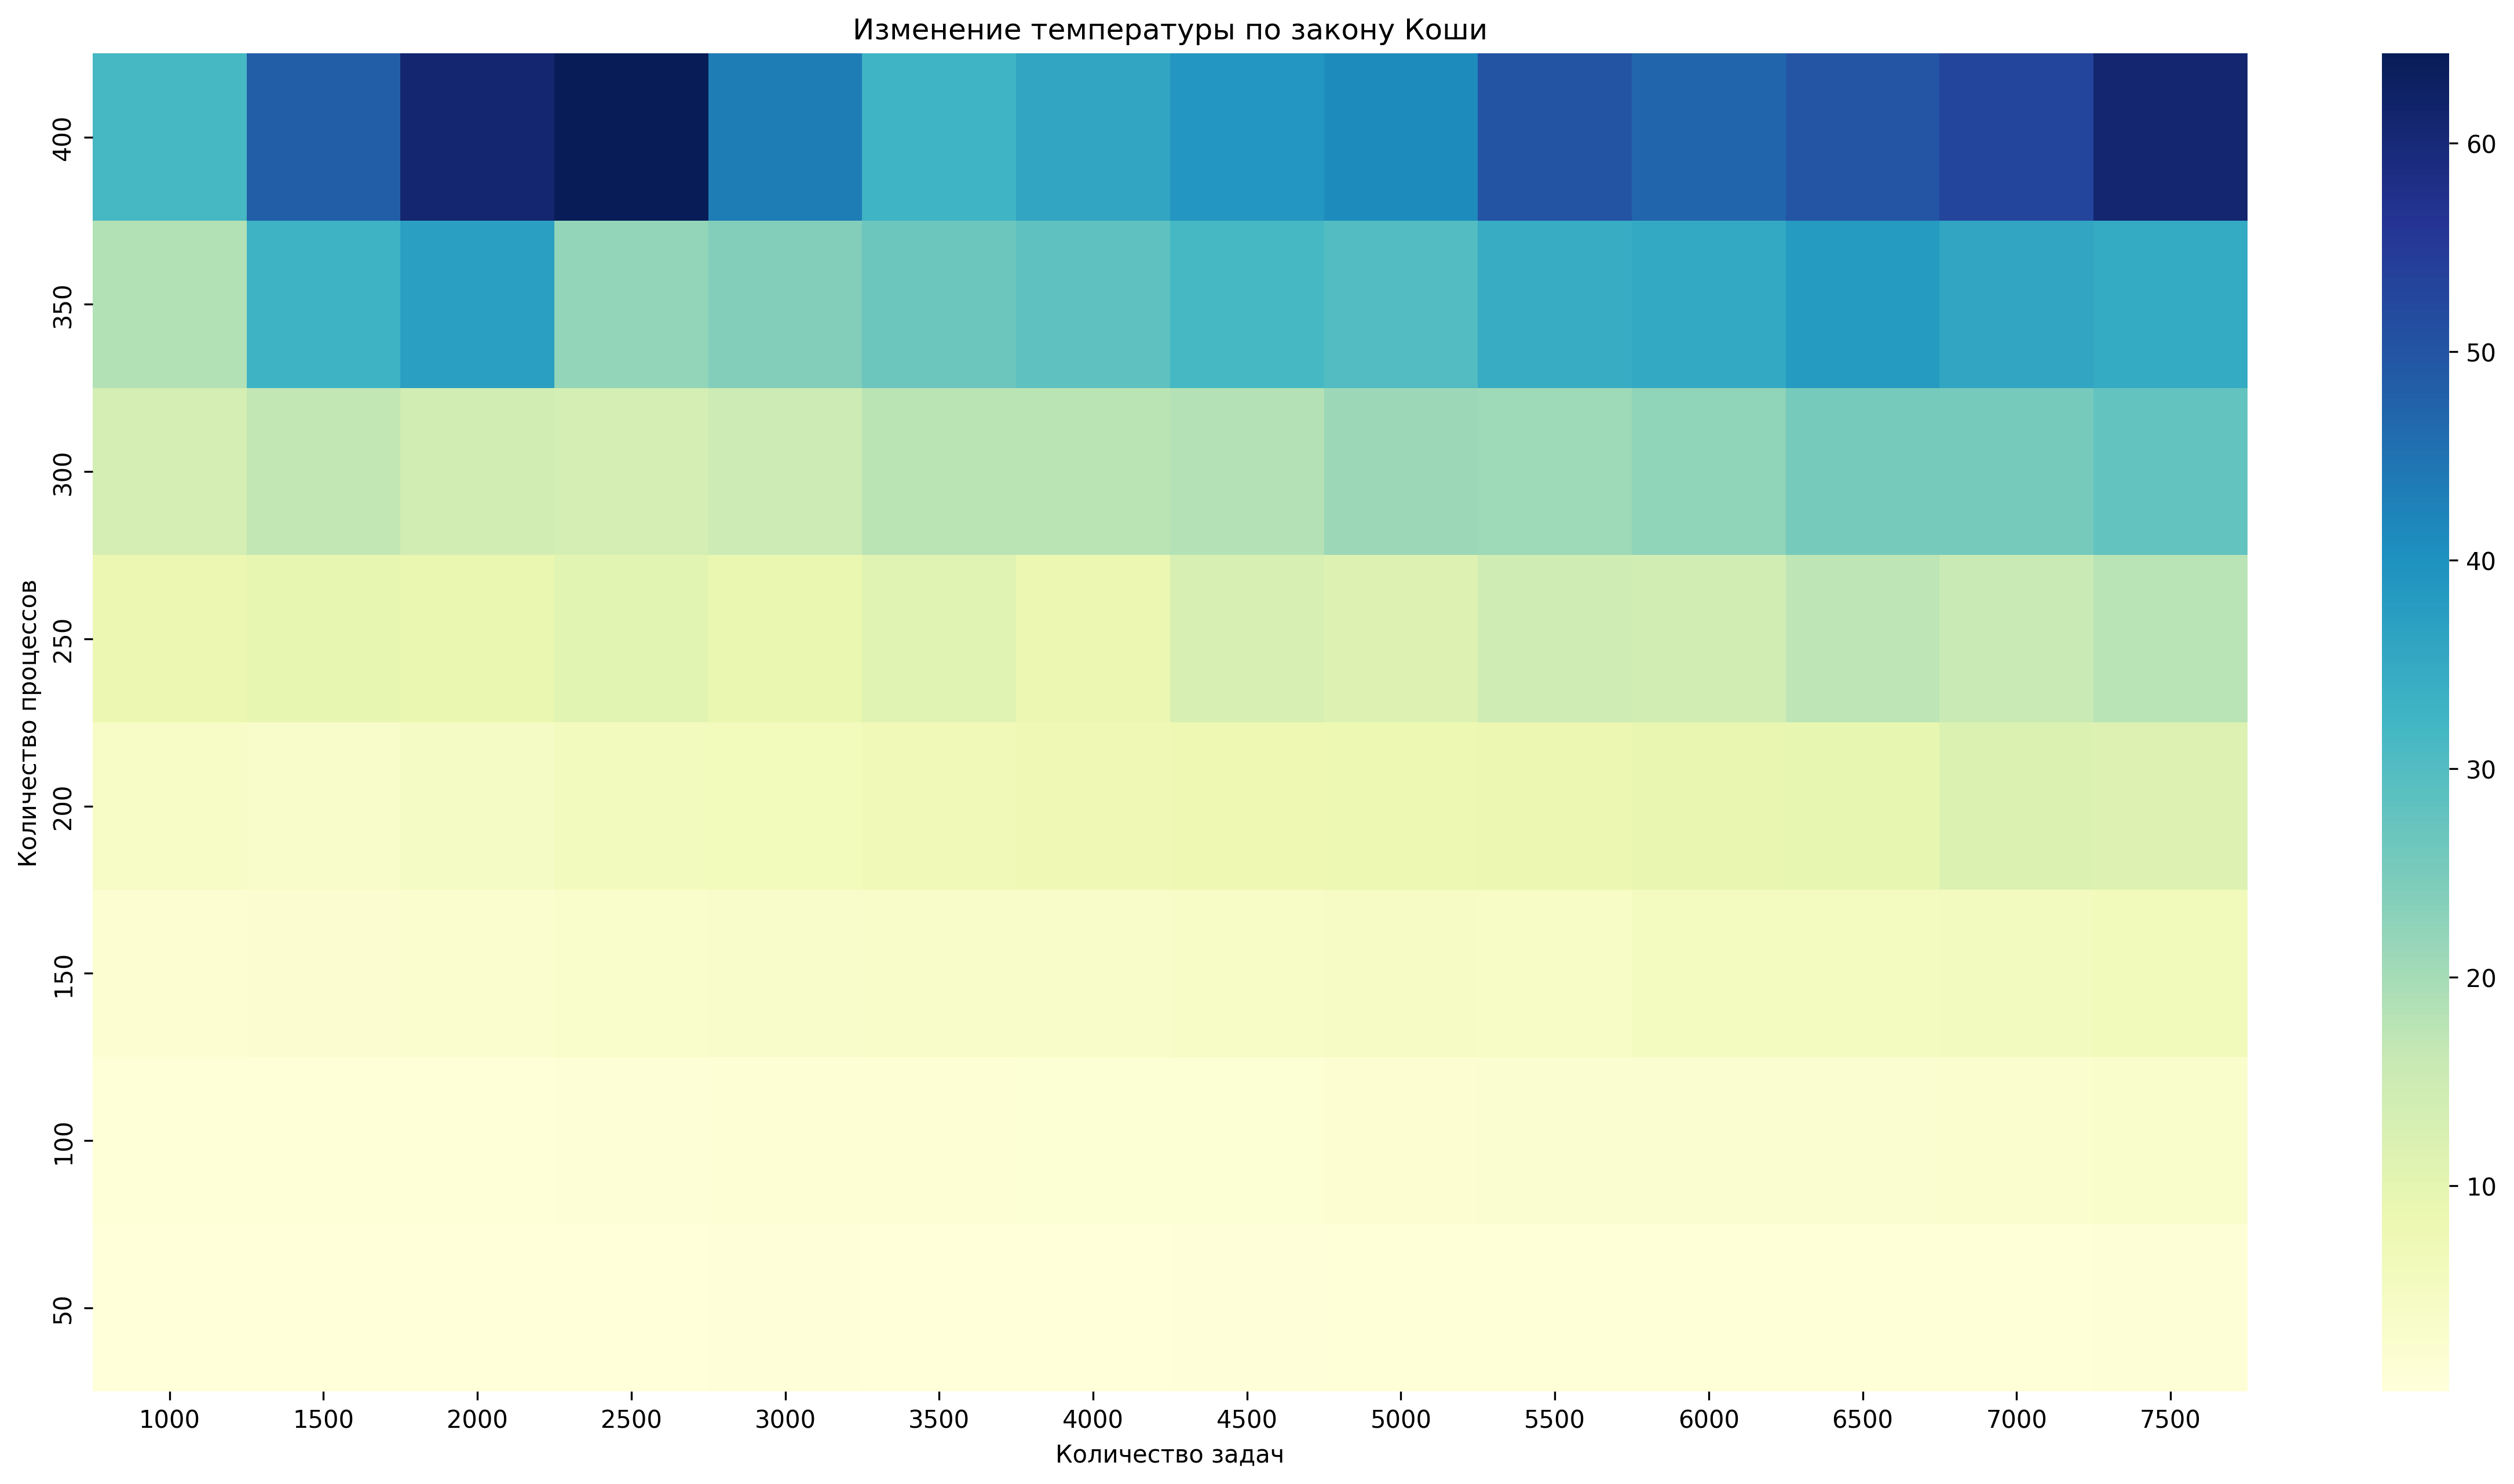
\includegraphics[width=0.8\linewidth]{Cauchy.png}
    \caption{По закону Коши}
    \label{fig:enter-label}
\end{figure}

\begin{figure}[!h]
    \centering
    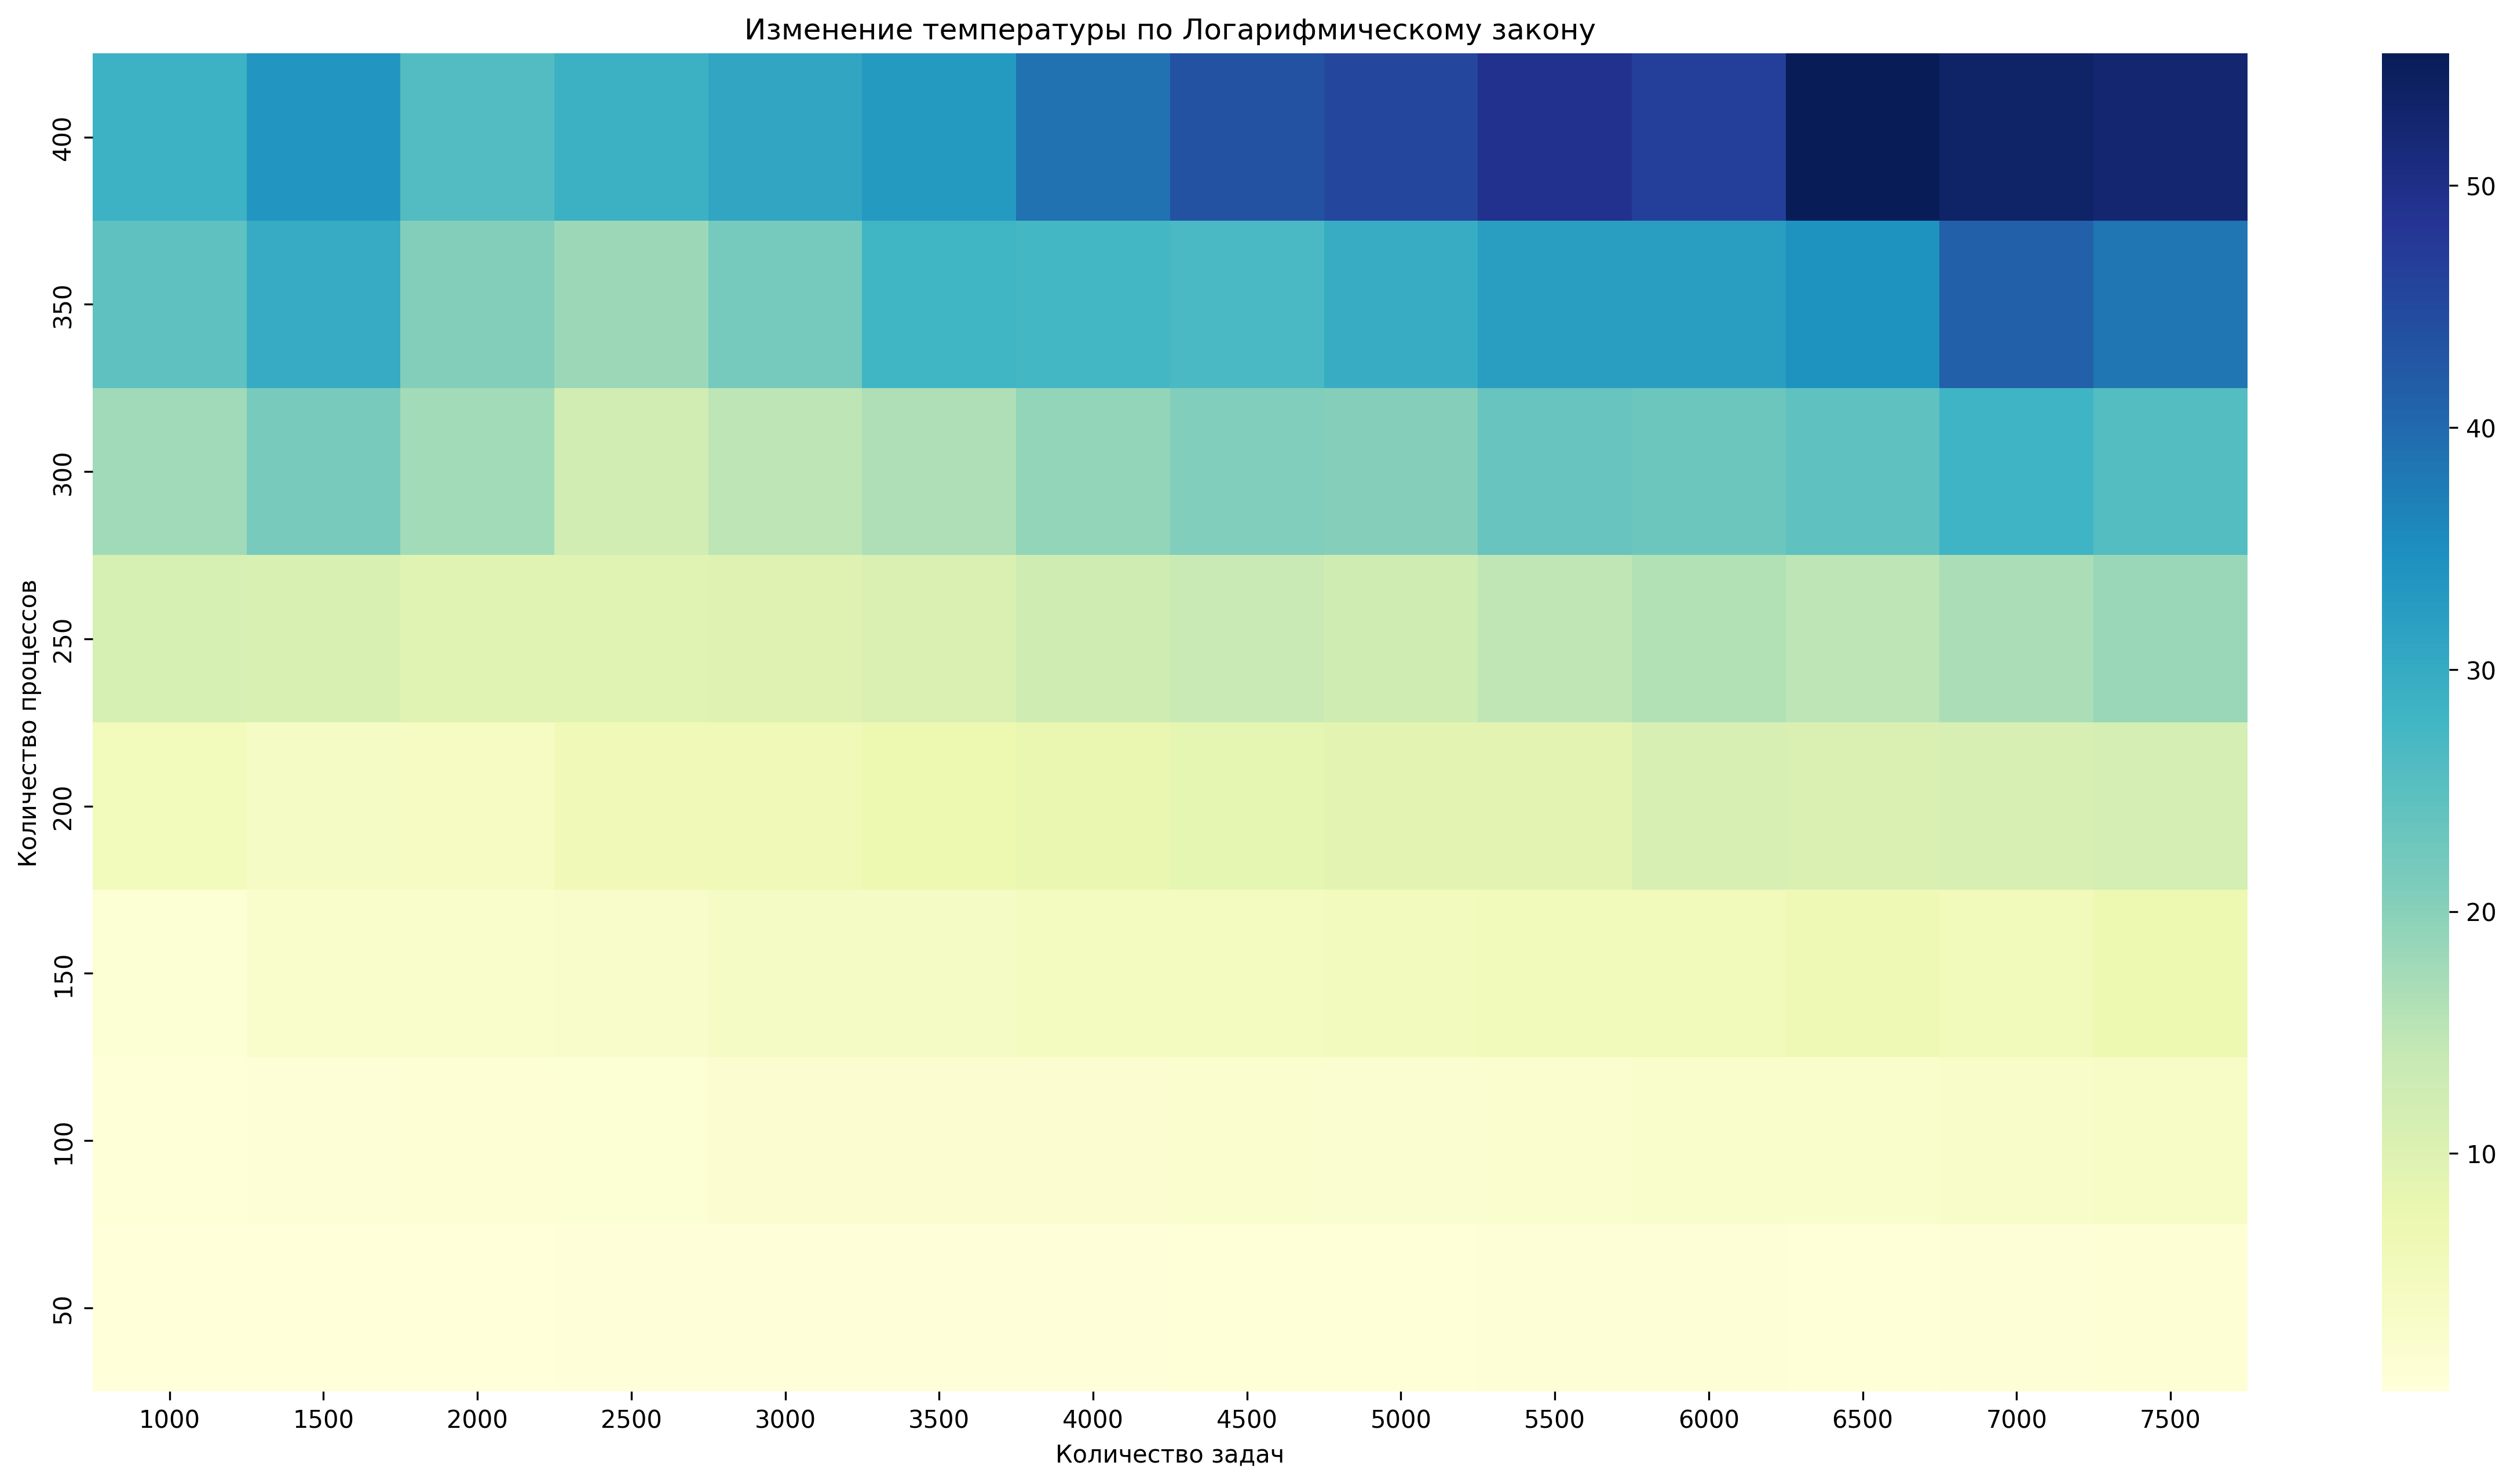
\includegraphics[width=0.8\linewidth]{Log-3.png}
    \caption{По Логарифмическому закону}
    \label{fig:enter-label}
\end{figure}

\newpage

Исходя из полученных графиков можно сделать вывод, что время выполнения распределения растет при росте количества процессоров и количества задач. Дольше всего работает закон Больцмана  и при этом показывает не самое лучшее значение критерия. Быстрее всех работает Логарифмический закон и имеет точность, схожую с законом Коши.

\subsection{Исследование параллельной реализации}

Схема работы параллельного алгоритма имеет практически следующий вид(рис. 3), но только у всех потоков будет одинаковое начальное решение.

\begin{figure}[!h]
    \centering
    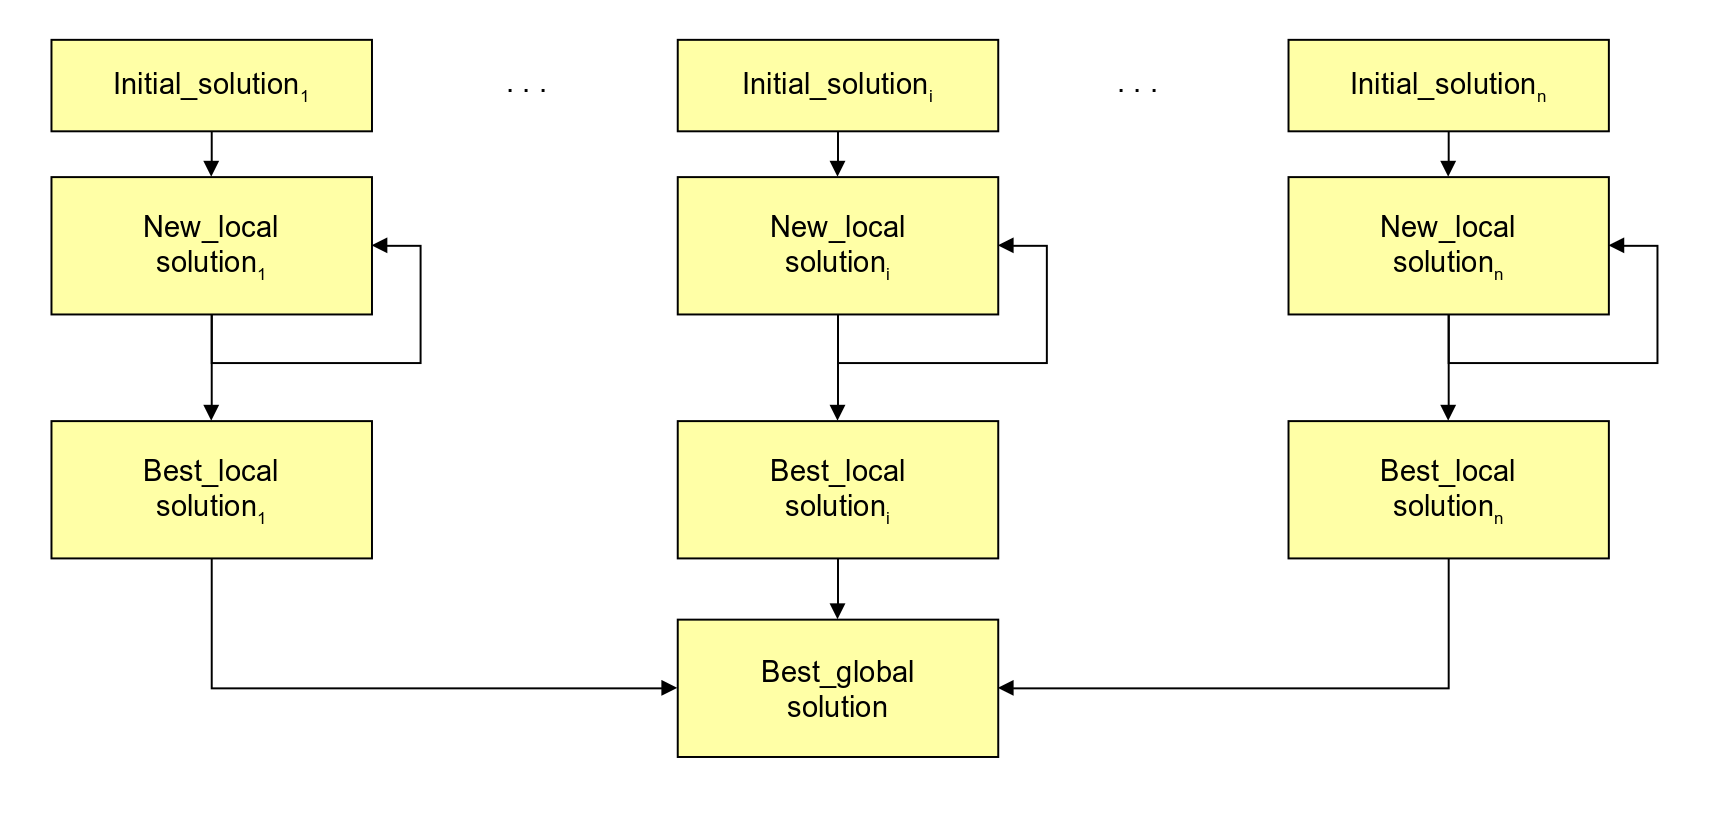
\includegraphics[width=1\linewidth]{Снимок экрана 2024-11-04 в 13.41.24.png}
    \caption{Параллельная реализация}
    \label{fig:enter-label}
\end{figure}

\newpage

Была проведена серия экспериментов для двух типов задач (100 задач и 20 процессов , 7500 задач и 400 процессов). В первом случае было проведено по 100 запусков программы, во втором по 10, так как каждый запуск работал около 1 минуты. Реализация получилась такой, что нет никакого выигрыша по времени программы, при любом количестве потоков программа будет работать приблизительно одинаково, при этом явно видно, что при росте количества потоков качество становится лучше. В связи с этим предлагается использовать именно параллельную реализацию, а не последовательную.

\begin{figure}[h]
\begin{minipage}[h]{0.47\linewidth}
\center{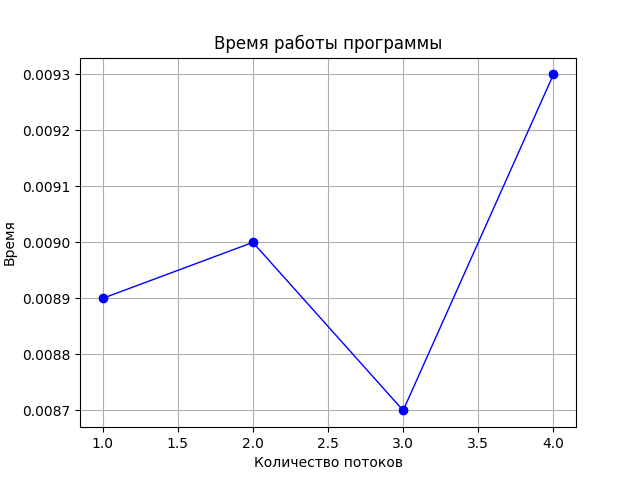
\includegraphics[width=1\linewidth]{time1.png}} a) \\
\end{minipage}
\hfill
\begin{minipage}[h]{0.47\linewidth}
\center{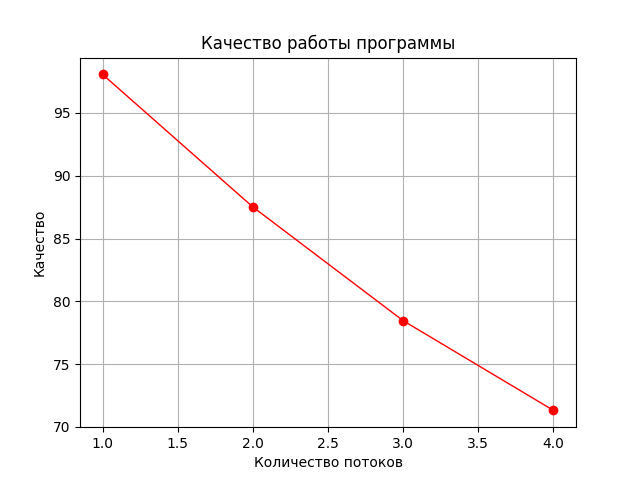
\includegraphics[width=1\linewidth]{Kach1.png}} \\b)
\end{minipage}
\vfill
\begin{minipage}[h]{0.47\linewidth}
\center{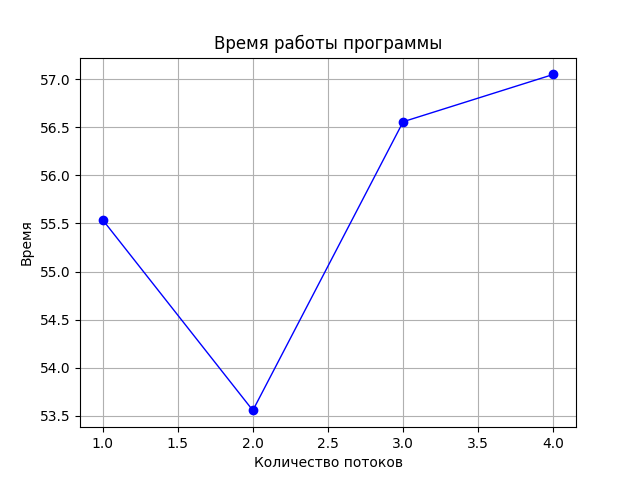
\includegraphics[width=1\linewidth]{time2.png}} c) \\
\end{minipage}
\hfill
\begin{minipage}[h]{0.47\linewidth}
\center{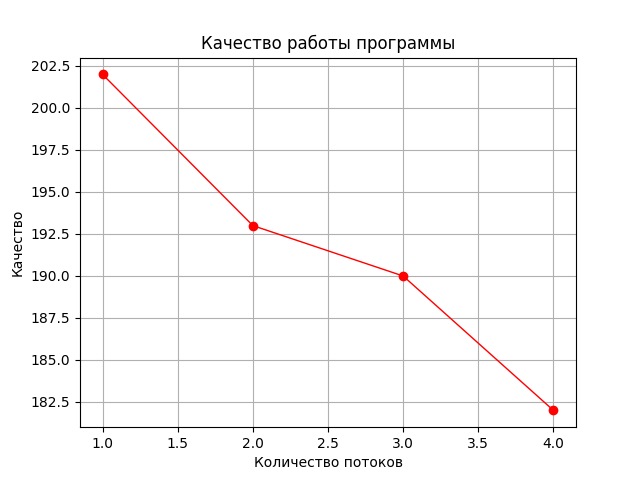
\includegraphics[width=1\linewidth]{Kach2.png}} d) \\
\end{minipage}
\caption{Результаты работы параллельного алгоритма (время и качество) при 100 задачах и 20 проыцессах (a и b) и при 7500 задачах и 400 процессах (c и d)}
\label{ris:experimentalcorrelationsignals}
\end{figure}


\end{document}
